\chapter{Transformacja Hough'a}
\label{sec:hough}

Transformacja Hough'a (czyt. Hafa) wykorzystywana jest w~procesie analizy obrazów i~służy do wykrywania na nim kształtów parametrycznych oraz nieparametrycznych w~zależności od jej wariantu \cite{mukhopadhyay2015survey}. Samo pojęcie transformacji odnosi się do odwzorowywania pojedynczych pikseli obrazu binarnego lub ich zbioru w~procesie głosowania w~przestrzeni akumulatora. Obraz wejściowy wcześniej poddany być musi procesowi wykrywania krawędzi. Dane zebrane w~akumulatorze biorą następnie udział w~procesie, w~którym wyłonione zostają potencjalne kształty poprzez wykrywanie największych wartości w~akumulatorze. W~zależności od specyfiki problemu oraz wykrywanych kształtów wykrywanie maksimów może odbywać się na różne sposoby. Użyte może zostać proste progowanie, wykrywanie i~uśrednianie skupisk, czy też filtracja przestrzeni akumulatora. Ogólny schemat przetwarzania przedstawiony jest na rysunku~\ref{fig:hough}.

\begin{figure}
    \centering
    \begin{tikzpicture}


\node[draw, rectangle, minimum height=0.9cm] (e) {Edge detection};
\node[draw, rectangle, minimum height=0.9cm, right=0.9cm of e] (t) {Hough transform};
\node[draw, rectangle, minimum height=0.9cm, right=0.9cm of t] (v) {Voting};
\node[draw, rectangle, minimum height=0.9cm, right=0.9cm of v] (p) {Further processing};

\path [draw, latex-o, ultra thick] (e) -- node[right] {Input image} ++(0,2);
\path [draw, -latex, ultra thick] (e) -- node[right] {} (t);
\path [draw, -latex, ultra thick] (t) -- node[right] {} (v);
\path [draw, -latex, ultra thick] (v) -- node[right] {} (p);
\path [draw, -latex, ultra thick] (p) -- node[left] {Detected patterns} ++(0,2);

\end{tikzpicture}

    \caption{Ogólny schemat przetwarzania obrazu z~wykorzystaniem transformacji Hough'a.}
    \label{fig:hough}
\end{figure}

\section{Standard Hough Transform}

Pracą, która jako pierwsza opisała tę transformację jest zgłoszony w~1962r. patent Paula Hough'a \cite{hough1962method}. Opisał on wykrywanie linii poprzez zastosowanie odwzorowania PTLM (point-to-line mapping). Odwzorowanie to dla każdego piksela rysuje linię w~dwuwymiarowej przestrzeni akumulatora zgodnie z~kierunkowym równaniem prostej (\ref{eq:hough-1}) przekształconym do postaci (\ref{eq:hough-2}). Stosując odwzorowanie odwrotne dla punktów o~największych wartościach możemy otrzymać potencjalne linie na obrazie. Transformację stosującą pełne odwzorowanie wszystkich punktów obrazu na parametry kształtów nazywamy standardową transformacją Hough'a (Standard Hough Transform, SHT).
\begin{align}
    y(x) &= mx+c \label{eq:hough-1}\\
    c(m) &= -xm+y \label{eq:hough-2}
\end{align}
\begin{eqexpl}
    \item{$x, y$} współrzędne piksela na obrazie;
    \item{$m$} zbocze prostej;
    \item{$c$} punkt przecięcia prostej z~osią Y.
\end{eqexpl}

\begin{figure}
    \centering
    \begin{subfigure}{0.45\textwidth}
        \centering
        \begin{tikzpicture}[scale=0.9]
    \begin{scope}[yscale=-1] 
    \tkzInit[xmax=6.2,ymax=6.2,xmin=0,ymin=0]
    \tkzGrid[]
    \tikzset{xlabel style/.append style={above=5pt}}
    \tkzAxeXY[]
    \draw[gray, ultra thick] (-0.5,0.5) -- (5.5,6.5);
    \fill (0, 1)  circle[radius=2pt];
    \fill (1, 2)  circle[radius=2pt];
    \fill (2, 3)  circle[radius=2pt];
    \fill (3, 4)  circle[radius=2pt];
    \fill (4, 5)  circle[radius=2pt];
    \fill (5, 6)  circle[radius=2pt];
    \end{scope}
\end{tikzpicture}

    \caption{Binarny obraz wejściowy}\label{fig:houghSlopeA}
    \end{subfigure}\hfill
    \begin{subfigure}{0.45\textwidth}
        \centering
        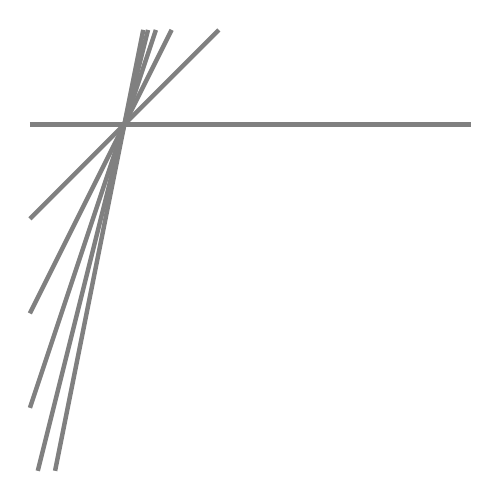
\begin{tikzpicture}[scale=0.8]
    \begin{scope}[yscale=-1] 
    \tkzInit[xmax=6,ymax=6,xmin=0,ymin=0]
    \tkzGrid[]
    \tikzset{xlabel style/.append style={above=5pt}}
    \tkzAxeXY[]
    \draw[gray, ultra thick] (-0.5,1) -- (6.5,1);
    \draw[gray, ultra thick] (-0.5,2.5) -- (2.5,-0.5);
    \draw[gray, ultra thick] (-0.5,4) -- (1.75,-0.5);
    \draw[gray, ultra thick] (-0.5,5.5) -- (1.5,-0.5);
    \draw[gray, ultra thick] (-0.375,6.5) -- (1.375,-0.5);
    \draw[gray, ultra thick] (-0.1,6.5) -- (1.3,-0.5);
    \end{scope}
\end{tikzpicture}

    \caption{Wynik transformacji}\label{fig:houghSlopeB}
    \end{subfigure}

    \caption{Demonstracja transformacji Hough'a w~wariancie równania kierunkowego prostej.}
    \label{fig:houghSlope}
\end{figure}
\hspace{1cm}


Na rysunku \ref{fig:houghSlope} przedstawiono obraz wejściowy (rys. \ref{fig:houghSlopeA}) oraz wynik transformacji (rys. \ref{fig:houghSlopeB}). Na rysunkach reprezentujących obraz oś Y jest skierowana w~dół, co ułatwia interpretację w~zgodności ze sposobem indeksowania pikseli obrazów podczas ich przetwarzania, gdzie punkt $(0,0)$ znajduje się w~lewym górnym rogu. W~wyniku transformacji każdy jasny piksel obrazu $(x, y)$ został odwzorowany na linię zgodnie z~równaniem (\ref{eq:hough-2}). Linie te przecięły się w~jednym punkcie $(1,1)$. W~wariancie dyskretnym transformacji wartość akumulatora w~punkcie $(1,1)$ miałaby największą wartość. W~tym wypadku punkt $(1,1)$ akumulatora przekłada się na prostą o~równaniu $y = x+1$, co zgadza się z~prostą na rysunku \ref{fig:houghSlopeA}.
\begin{wrapfigure}{r}{7cm}
    \centering
    

\begin{tikzpicture}[scale=0.9]

    \begin{scope}[yscale=-1] 
    \tkzInit[xmax=5.5,ymax=5.5,xmin=0,ymin=0]
    \tkzGrid[]
    \tikzset{xlabel style/.append style={above=5pt}}
    \tkzAxeXY
    \tkzClip[space=1]

    \draw[gray, ultra thick] (-0.5 ,5.5) -- (5.5,-0.5);

    \fill (0, 5)  circle[radius=2pt];
    \fill (1, 4)  circle[radius=2pt];
    \fill (2, 3)  circle[radius=2pt];
    \fill (3, 2)  circle[radius=2pt];
    \fill (4, 1)  circle[radius=2pt];
    \fill (5, 0)  circle[radius=2pt];

    \tkzDefPoints{0/0/O,2.5/2.5/B,5/0/A}
    \tkzMarkAngle[size=0.5](A,O,B)
    \tkzFillAngle[size=0.5,fill=red!20, opacity=0.5](A,O,B)
    \tkzLabelAngle(A,O,B){$\theta$}

    \tkzMarkRightAngle[german, size=0.45](O,B,A)

    \draw[gray, thick, dashed] (0,0) -- (2.5,2.5) node [midway, right, color=black] {$\rho$}; ;
\end{scope}

\end{tikzpicture}

    \caption{Prosta opisana za pomocą odległości $\rho$ i~kąta $\theta$ od środka układu współrzędnych biegunowych.}
    \label{fig:houghLineAngle}
\end{wrapfigure}




Taka reprezentacja punktu w~przestrzeni akumulatora rodzi jednak problem w~przypadku wykrywania linii pionowych. Piksele obrazu zorientowane w~pionie w~przestrzeni akumulatora utworzą linie równoległe. Brak punktu przecięcia takich linii uniemożliwia wykrycie linii na obrazie. Rozwiązaniem tego problemu jest zaproponowana w~1972 roku zmiana reprezentacji prostej, gdzie zamiast zbocza i~punktu przecięcia z~osią Y użyto biegunowego układu współrzędnych oraz prostej normalnej do wykrywanej prostej \cite{duda1972use}. Przykładowa prosta została zaprezentowana na rysunku \ref{fig:houghLineAngle} i~reprezentowana jest przez wartości odległości $\rho=\frac{5\sqrt{2}}{2}$ i~kąta obrotu $\theta=\frac{\pi}{4}$ wokół środka układu współrzędnych. Prosta odwzorowywana jest na sinusoidę zgodnie z~równaniem \ref{eq:sinCos}.
\begin{align}
    \rho(\theta) &= x\cos{\theta} + y\sin{\theta} \label{eq:sinCos}
\end{align}
\begin{eqexpl}
    \item{$x, y$} współrzędne piksela na obrazie;
    \item{$\rho$} odległość prostej od środka układu współrzędnych;
    \item{$\theta$} obrót prostej od wokół układu współrzędnych.
\end{eqexpl}

Na rysunku \ref{fig:houghSinCos} przedstawiono zawartość akumulatora po transformacji obrazu z~rysunku \ref{fig:houghSlopeA}. Zgodnie z~oczekiwaniami sinusoidy te przecinają się w~punktach, które reprezentują wykryte linie. Dwa punkty $(\frac{3\pi}{4}, \frac{\sqrt{2}}{2})$ oraz $(\frac{7\pi}{4}, -\frac{\sqrt{2}}{2})$, z~racji na okresowość funkcji trygonometrycznych reprezentują tę samą linię. Przestrzeń akumulatora dla kąta obrotu można zatem ograniczyć do $\theta \in \left[ 0, \pi\right)$ \cite{immerkaer1998some}.

\begin{figure}[t]
    \centering
    \begin{tikzpicture}[]
    \tkzInit[xmax=360,xstep=30,ymax=3,xmin=0,ymin=-3]
    \tkzGrid[]
    \tkzClip[space=0.75]
    \tkzDrawX[label=$\theta$]
    \tkzLabelX
    \tkzDrawY[label=$\rho$]
    \tkzLabelY

    \draw plot[domain=0:360/30,smooth] (\x,{0*cos(\x*30*0.0174532925 r) + 1*sin(\x*30*0.0174532925 r)});
    \draw plot[domain=0:360/30,smooth] (\x,{1*cos(\x*30*0.0174532925 r) + 2*sin(\x*30*0.0174532925 r)});
    \draw plot[domain=0:360/30,smooth] (\x,{2*cos(\x*30*0.0174532925 r) + 3*sin(\x*30*0.0174532925 r)});
    \draw plot[domain=0:360/30,smooth] (\x,{3*cos(\x*30*0.0174532925 r) + 4*sin(\x*30*0.0174532925 r)});
    \draw plot[domain=0:360/30,smooth] (\x,{4*cos(\x*30*0.0174532925 r) + 5*sin(\x*30*0.0174532925 r)});
    \draw plot[domain=0:360/30,smooth] (\x,{5*cos(\x*30*0.0174532925 r) + 6*sin(\x*30*0.0174532925 r)});
\end{tikzpicture}

    \caption{Wynik transformacji Hough'a dla obrazu na rysunku \ref{fig:houghSlopeA} w~wariancie współrzędnych biegunowych.}
    \label{fig:houghSinCos}
\end{figure}


W czasie transformacji, na końcowy rezultat mają wpływ szumy, które powstały na skutek niedoskonałości procesu wykrywania krawędzi, są bardzo krótkimi krawędziami lub są krawędziami, ale nieuwzględnianymi w~rozwiązywanym problemie. Przykładem mogą być okręgi podczas wykrywania linii na obrazie. Proces głosowania w~przestrzeni akumulatora musi uwzględniać takie sytuacje i~proste progowanie może zostać zastąpione bardziej złożonymi metodami \cite{palmer1997optimizing, perantonis1998robust}.

Na potrzeby prowadzonych badań zaimplementowany został algorytm wykrywania prostych na~obrazie binarnym, który jako wykrywanie maksimów w~akumulatorze wykorzystuje proste progowanie.

\section{Circle Hough Transform}

Prosta do swojej reprezentacji potrzebuje dwóch parametrów - zbocza i~punktu przecięcia z~osią Y. Okrąg natomiast jest kształtem parametrycznym, które potrzebuje trzech parametrów - współrzędnych środka i~promienia. Idąc dalej, możemy rozszerzać liczbę parametrów, zyskując możliwość stosowania transformacji Hough'a do wykrywania coraz bardziej skomplikowanych kształtów.

Akumulator w~Circle Hough Transform (CHT) ma trzy wymiary, po jednym na każdy parametr tak samo jak w~SHT, która do wykrywania linii wykorzystywała dwuwymiarowy akumulator. Dla każdego z~możliwych promieni, dla każdego piksela obrazu w~przestrzeni akumulatora rysujemy okrąg, którego ten piksel jest środkiem. Efektywnie jeden piksel obrazu mapowany jest na stożek w~trójwymiarowej przestrzeni akumulatora. Na rysunku \ref{fig:houghCircleStandard} przedstawiono przykładowe okręgi  w~dwóch wymiarach dla stałego promienia. Wszystkie te narysowane okręgi przecinają się w~środku właściwego okręgu \cite{mukhopadhyay2015survey}. W~takiej trójwymiarowej przestrzeni akumulatora jego największe wartości wskazywać będą na konkretne środki oraz promienie potencjalnych okręgów na obrazie wejściowym.

\begin{figure}
    \centering
    \begin{subfigure}{0.45\textwidth}
        \centering
        \begin{tikzpicture}[scale=0.9]
    \begin{scope}[yscale=-1] 
    \tkzInit[xmax=6.2,ymax=6.2,xmin=0,ymin=0]
    \tkzClip[space=1]
    \tkzGrid[]
    \tikzset{xlabel style/.append style={above=5pt}}
    \tkzAxeXY[]


        \tkzDefPoints{3/3/O,3/5/C}
        \tkzDefCircle[through](O,C)
        \tkzGetLength{rOC}
        \tkzDrawCircle[dashed](O,C)
        \tkzDrawPoints(O)
    
        \tkzDefPoints{3/1/B}
        \tkzGetLength{rOB}
        \tkzDefCircle[through](B,O)
        \tkzDrawPoints(B)
        \tkzDrawCircle(B,O)

        \tkzDefPoints{5/3/B}
        \tkzGetLength{rOB}
        \tkzDefCircle[through](B,O)
        \tkzDrawPoints(B)
        \tkzDrawCircle(B,O)

        \tkzDefPoints{3/5/B}
        \tkzGetLength{rOB}
        \tkzDefCircle[through](B,O)
        \tkzDrawPoints(B)
        \tkzDrawCircle(B,O)

        \tkzDefPoints{1/3/B}
        \tkzGetLength{rOB}
        \tkzDefCircle[through](B,O)
        \tkzDrawPoints(B)
        \tkzDrawCircle(B,O)

    
    \end{scope}
\end{tikzpicture}

        \caption{CHT dla stałego promienia w~wariancie standardowym.}
        \label{fig:houghCircleStandard}
    \end{subfigure}\hfill
    \begin{subfigure}{0.45\textwidth}
        \centering
        \begin{tikzpicture}[scale=0.9]
    \begin{scope}[yscale=-1]
    \tkzInit[xmax=6.2,ymax=6.2,xmin=0,ymin=0]
    \tkzClip[space=1]
    \tkzGrid[]
    \tikzset{xlabel style/.append style={above=5pt}}
    \tkzAxeXY[]

        \tkzDefPoints{3/3/O,3/5/C}
        \tkzDefCircle[through](O,C)
        \tkzGetLength{rOC}
        \tkzDrawCircle[dashed](O,C)
        \tkzDrawPoints(O)
    
        \tkzDefPoint(3,3){A}\tkzDefPoint(0,0){O}
        \tkzDefShiftPoint[A](0:4){B}
        \tkzDefShiftPoint[A](90:4){C}
        \tkzDefShiftPoint[A](180:4){D}
        \tkzDefShiftPoint[A](270:4){E}
        \tkzDefShiftPoint[A](45:4){F}
        \tkzDefShiftPoint[A](135:4){G}
        \tkzDefShiftPoint[A](225:4){H}
        \tkzDefShiftPoint[A](-45:4){I}
        \tkzDrawSegments[ultra thick, opacity=0.5](A,B A,C A,D A,E A,F A,G A,H A,I)
  
    
    \end{scope}
\end{tikzpicture}

        \caption{CHT w~wariancie gradientowym dla wybranych kierunków.}
        \label{fig:houghCircleGradient}
        \vfill
    \end{subfigure}
    \caption{Wynik transformacji}\label{fig:houghCircle}
\end{figure}

\subsection{Wariant z~wykorzystaniem gradientu}

Wraz ze skomplikowaniem kształtu parametrycznego rośnie liczba jego parametrów, których liczba stanowi liczbę wymiarów akumulatora. Dla każdego jasnego piksela obrazu konieczne jest uaktualnienie akumulatora we wszystkich jego wymiarach, co prowadzi do zwiększenia wykładniczej złożoności obliczeniowej. Dlatego dąży się do redukcji wymiarowości problemu zazwyczaj łącząc przetwarzanie charakterystyczna dla SHT z~dodatkową informacją z~przestrzeni obrazu. Biblioteka OpenCV implementuje mniej złożony wariant transformacji \cite{ito2012detection}, który oparty jest na wykorzystaniu gradientu wykrytych krawędzi. W~wariancie tym najpierw w~dwuwymiarowym akumulatorze następuje głosowanie nad centrum potencjalnego okręgu.

W pierwszej kolejności binarny obraz poddawany jest operacji splotu z~filtrem Sobela osobno w~kierunku pionowym oraz poziomym. Pozwala to na uzyskanie pochodnych cząstkowych w~danym punkcie, które razem tworzą gradient, czyli prostopadły kierunek przebiegu krawędzi potencjalnie wskazujący środek wyszukiwanego okręgu. W~dwuwymiarowym akumulatorze od analizowanego punktu w~dwóch kierunkach rysowana jest linia o~długości maksymalnego poszukiwanego promienia. W~przypadku okręgu wszystkie te linie przecinają się w~jednym punkcie, co pokazane zostało na rysunku \ref{fig:houghCircleGradient}. Kolejnym krokiem jest wykrycie maksimów w~akumulatorze. Aby zmniejszyć szumy i~liczbę okręgów leżących blisko siebie, po procesie progowania środki leżące bliżej siebie niż ustalona odległość są łączona w~jeden. Następnie dla każdego punktu po wykryciu maksimów w~akumulatorze, w~drugim jednowymiarowym akumulatorze, dla każdego możliwego poszukiwanego promienia następuje głosowanie. Zliczana jest liczba jasnych pikseli obrazu, które znajdują się w~danej odległości od środka, co po wykryciu maksimum w~akumulatorze uzupełnia dane okręgu o~najbardziej prawdopodobny promień.

Na potrzeby prowadzonych badań zaimplementowany został algorytm wykrywania okręgów na~obrazie binarnym, który wykorzystuje metodą gradientów oraz jako wykrywanie maksimów w~akumulatorze podczas głosowania dla środków jak i~promieni wykorzystuje proste progowanie.

\subsection{Próbkowanie i~złożoność obliczeniowa}

Głównym elementem wpływającym na złożoność obliczeniową transformacji Hough'a jest liczba analizowanych parametrów kształtów. Dla SHT złożoność wynosi $O(n)$ dla procesu głosowania i~$O(S_\rho S_\theta)$ dla procesu wykrywania maksimum, gdzie $n$ jest liczbą jasnych pikseli obrazu, a~$S_\rho$ i~$S_\theta$ parametrami próbkowania parametrów w~przestrzeni akumulatora. Widać zatem, że złożoność w~tym wypadku zależy od jakości danych wejściowych, gdzie wszelkie szumy zwiększają czas wykonania algorytmu. Kolejnym elementem jest próbkowanie w~przestrzeni akumulatora. Zwiększenie próbkowania pozwala uzyskać większą precyzję detekcji, ale zwiększa liniowo (dla jednego wymiaru) rozmiar akumulatora, a~co za tym idzie ilość obliczeń wymaganych w~procesie głosowania. Ważnym czynnikiem jest specyfika problemu, który rozwiązywać ma transformacja Hough'a. Możemy zmniejszyć czas wykonania algorytmu ograniczając zakres poszukiwań głosując w~ustalonej podprzestrzeni akumulatora, na przykład analizując linie nachylone tylko pod określonym zakresem kątów i~leżące w~danej odległości od punktu odniesienia.

Transformacja Hough'a użyta została w~algorytmach wspólnych dla wszystkich testów w~środowiskach, które zostały przystosowane do badanych metod akceleracji. Wybrana została do tego celu ze względu na swoją złożoność obliczeniową, podział na wiele etapów oraz, w~wariancie SHT, wykorzystania funkcji trygonometrycznych. Operuje ona również na dużych zbiorach danych, co dodatkowo pozwala rzucić światło na konieczność zarządzania pamięcią i~transferu danych dla wybranych metod akceleracji. 
